\section{Results}
%---------------------------------------------------------------------------------------------------
\subsection{Risk Group Duration}\label{res.yss}
Figure~\ref{fig:yss.adj} illustrates
the estimated cumulative distributions for years selling sex
following each stage of adjustment outlined in \sref{meth.yss};
Table~\ref{tab:yss.adj} provides the corresponding distribution means(95\%~CI).
Ironically, the final estimate of 4.52 was similar to the original median of 4,
as each adjustment alternated betwen increasing and decreasing
the estimated distribution mean.
The censoring adjustment yielded the largest increase, while
the measurement adjustment yielded the largest decrease.
\begin{figure}
  \centering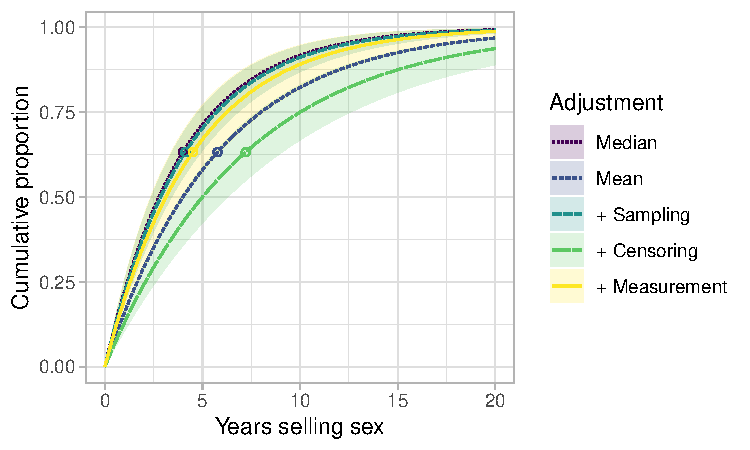
\includegraphics[scale=.75]{yss.adj}
  \caption{Estimated cumulative exponential distribution for years selling sex
    following each stage of adjustment}
  \label{fig:yss.adj}
  \floatfoot{
    Data from FSW in Eswatini (2011) \cite{Baral2014};
    lines: estimate; transparent ribbon: 95\%~CI; circles: distribution mean.}
\end{figure}
%---------------------------------------------------------------------------------------------------
\subsection{Sexual Partnership Duration}\label{res.partners}
% infer adjusted partnership Q, K & compare to naive estimates
\begin{figure}[h]
  \centering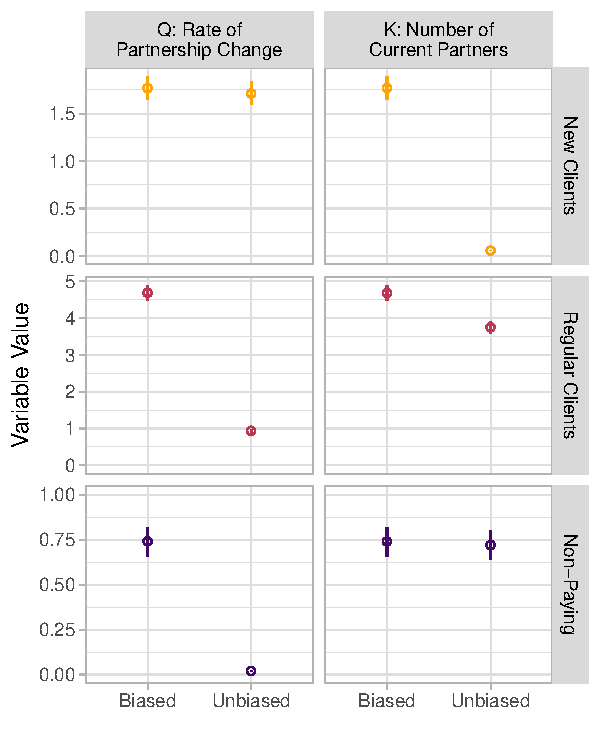
\includegraphics[scale=.8]{partners.fsw}
  \caption{Biased vs unbiased estimates of:
    number of current partners and rate of partnership change,
    for three partnership types reported by female sex workers in \cite{Baral2014}.
    Error bars show 95\%~CI from 10,000 simulated surveys with $N = 328$.}
  \label{fig:partners.fsw}
\end{figure}
\begin{figure}[h]
  \centering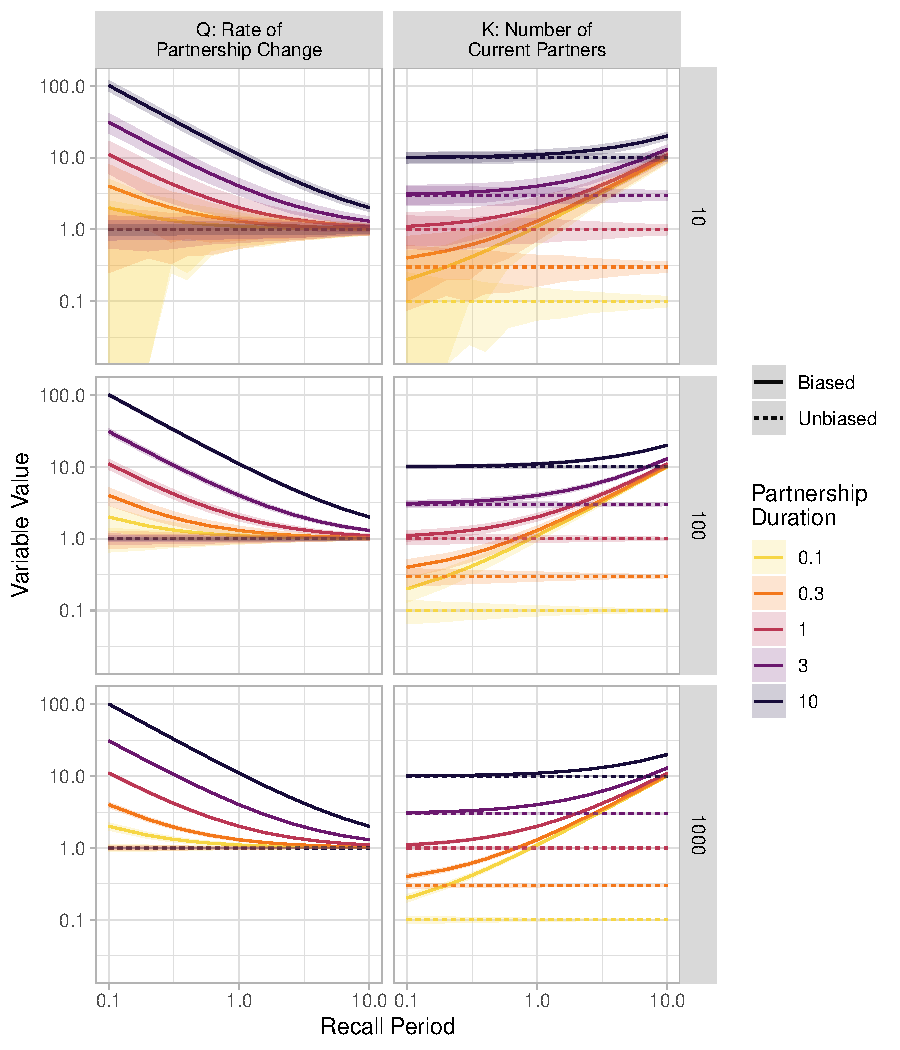
\includegraphics[scale=.8]{partners.sens}
  \caption{Biased vs unbiased estimates of:
    number of current partners and rate of partnership change,
    for different recall periods and partnership durations.
    Ribbons show 95\%~CI from 10,000 simulated surveys with $N = 10, 100, 1000$.}
  \label{fig:partners.sens}
\end{figure}
